\documentclass[twocolumn,twocolappendix,linenumbers]{aastex631}

\usepackage[dvipsnames]{xcolor}
\definecolor{linkcolor}{rgb}{0.1, 0.5, 0.7}

\usepackage{acronym}
\usepackage{lmodern}

\usepackage{amssymb}
\usepackage{amsmath}
\usepackage{physics}
\usepackage{orcidlink}
\usepackage{xspace}
\usepackage[normalem]{ulem}

\usepackage{eso-pic}

\newacro{PE}[PE]{parameter estimation}
\newacro{GW}[GW]{gravitational-wave}
\newacro{GWTC-3}[GWTC-3]{third gravitational-wave transient catalog}
\newacro{GWTC-2}[GWTC-2]{second gravitational-wave transient catalog}
\newacro{GWTC-4}[GWTC-4.0]{Fourth Gravitational-Wave Transient Catalog}
\newacro{GWTC-5}[GWTC-5.0]{Fifth Gravitational-Wave Transient Catalog}
\newacro{GWTC}[GWTC]{gravitational wave transient catalog}
\newacro{LVK}[LVK]{LIGO-Virgo-Kagra collaboration}
\newacro{O4}[O4]{fourth observing run}
\newacro{O3}[O3]{third observing run}
\newacro{HMC}[HMC]{Hamiltonian Monte Carlo}
\newacro{MC}[MC]{Monte Carlo}
\newacro{NUTS}[NUTS]{No-U-Turn Sampler}
\newacro{IID}[IID]{identically and independently distributed}
\newacro{CDF}[CDF]{Cumulative Distribution Function}
\newacro{SFR}[SFR]{star formation rate}
\newacro{KDE}[KDE]{kernel density estimate}
\newacro{BBH}[BBH]{binary black-hole}
\newacro{BNS}[BNS]{binary neutron star}
\newacro{NSBH}[NSBH]{neutron star-black hole binary}
\newacro{NS}[NS]{neutron star}
\newacro{BH}[BH]{black hole}
\newacro{PISN}[PISN]{pair-instability supernova}

\newacro{PPC}[PPC]{posterior predictive check}
\newacro{MI}[MI]{mutual information}
\newacro{CAR}[CAR]{conditional autoregressive}
\newacro{ICAR}[ICAR]{intrinsic conditional autoregressive}
\newacro{PDF}[PDF]{probability density function}
\newacro{KL}[KL]{Kullback--Leibler}
\newacro{JS}[JS]{Jensen--Shannon}

\newacro{XLA}[XLA]{Accelerated Linear Algebra}
\newacro{HLV}[HLV]{Hanford, Livingston and Virgo}
\newacro{SNR}[SNR]{signal-to-noise ratio}
\newacro{IID}[IID]{independent and identically distributed}
\newacro{PSD}[PSD]{power spectral density}
\newacro{DAG}[DAG]{directed acyclic graph}

\newacro{CE}[CE]{common-envelope}
\newacro{OC}[OC]{open cluster}
\newacro{NSC}[NSC]{nuclear star cluster}
\newacro{CHE}[CHE]{chemically-homogeneous evolution}
\newacro{GC}[GC]{globular cluster}
\newacro{AGN}[AGN]{active galactic nuclei}
\newacro{SMT}[SMT]{stable mass transfer}

\usepackage{dashrule}
\usepackage[absolute,overlay]{textpos}

\newacro{PE}[PE]{parameter estimation}
\newacro{GW}[GW]{gravitational-wave}
\newacro{GWTC-3}[GWTC-3]{third gravitational-wave transient catalog}
\newacro{GWTC-2}[GWTC-2]{second gravitational-wave transient catalog}
\newacro{GWTC-4}[GWTC-4.0]{Fourth Gravitational-Wave Transient Catalog}
\newacro{GWTC-5}[GWTC-5.0]{Fifth Gravitational-Wave Transient Catalog}
\newacro{GWTC}[GWTC]{gravitational wave transient catalog}
\newacro{LVK}[LVK]{LIGO-Virgo-Kagra collaboration}
\newacro{O4}[O4]{fourth observing run}
\newacro{O3}[O3]{third observing run}
\newacro{HMC}[HMC]{Hamiltonian Monte Carlo}
\newacro{MC}[MC]{Monte Carlo}
\newacro{NUTS}[NUTS]{No-U-Turn Sampler}
\newacro{IID}[IID]{identically and independently distributed}
\newacro{CDF}[CDF]{Cumulative Distribution Function}
\newacro{SFR}[SFR]{star formation rate}
\newacro{KDE}[KDE]{kernel density estimate}
\newacro{BBH}[BBH]{binary black-hole}
\newacro{BNS}[BNS]{binary neutron star}
\newacro{NSBH}[NSBH]{neutron star-black hole binary}
\newacro{NS}[NS]{neutron star}
\newacro{BH}[BH]{black hole}
\newacro{PISN}[PISN]{pair-instability supernova}

\newacro{PPC}[PPC]{posterior predictive check}
\newacro{MI}[MI]{mutual information}
\newacro{CAR}[CAR]{conditional autoregressive}
\newacro{ICAR}[ICAR]{intrinsic conditional autoregressive}
\newacro{PDF}[PDF]{probability density function}
\newacro{KL}[KL]{Kullback--Leibler}
\newacro{JS}[JS]{Jensen--Shannon}

\newacro{XLA}[XLA]{Accelerated Linear Algebra}
\newacro{HLV}[HLV]{Hanford, Livingston and Virgo}
\newacro{SNR}[SNR]{signal-to-noise ratio}
\newacro{IID}[IID]{independent and identically distributed}
\newacro{PSD}[PSD]{power spectral density}
\newacro{DAG}[DAG]{directed acyclic graph}

\newacro{CE}[CE]{common-envelope}
\newacro{OC}[OC]{open cluster}
\newacro{NSC}[NSC]{nuclear star cluster}
\newacro{CHE}[CHE]{chemically-homogeneous evolution}
\newacro{GC}[GC]{globular cluster}
\newacro{AGN}[AGN]{active galactic nuclei}
\newacro{SMT}[SMT]{stable mass transfer}

\newcommand{\comment}[1]{}
\newcommand{\red}[1]{{\color{Red} #1}}
\newcommand{\sa}[1]{{\bf\color{Thistle}SA: #1}}
\renewcommand{\ij}[1]{{\color{Green} #1}}
\newcommand{\PixelPop}{\textsc{PixelPop}\xspace}
\newcommand{\PPMixture}{\textsc{PixelPop Mixture}\xspace}
% \newcommand{\Bsplines}{\textsc{B-Splines}\xspace}
% \newcommand{\BsplMixture}{\textsc{B-Splines Mixture}\xspace}
\newcommand{\Gwinferno}{\textsc{GWInferno}\xspace}
\newcommand{\GwinfMixture}{\textsc{GWInferno Mixture}\xspace}
\newcommand{\oneparpeak}{\textsc{One parametric peak}\xspace}
\newcommand{\twoparpeaks}{\textsc{Two parametric peaks}\xspace}
\newcommand{\gtwou}{\textsc{Gaussian+Two Uniform}\xspace}


\newcommand{\Msun}{\ensuremath{\mathrm{M}_\odot}\xspace}
\newcommand{\chieff}{\ensuremath{\chi_\mathrm{eff}}\xspace}


\begin{document}


\title{Bumps, bumps, and more bumps: Model-independent evidence for features in the primary mass distribution of the Binary Black Hole population}

\author{Sofía Álvarez-López\,\orcidlink{0009-0003-8040-4936}}\email{sofiaal@mit.edu}
\affiliation{LIGO Laboratory, Massachusetts Institute of Technology, Cambridge, MA 02139, USA}
\affiliation{Kavli Institute for Astrophysics and Space Research, Massachusetts Institute of Technology, Cambridge, MA 02139, USA}
\affiliation{Department of Physics, Massachusetts Institute of Technology, Cambridge, MA 02139, USA}

\author{Ivan Juarez Reyes}
\affiliation{Institute for Fundamental Science, University of Oregon, Eugene, OR 97403, USA}
\affiliation{Department of Physics and Astronomy, University of Oregon, Eugene, OR 97403, USA}

\author{Ben Farr}
\affiliation{Institute for Fundamental Science, University of Oregon, Eugene, OR 97403, USA}
\affiliation{Department of Physics and Astronomy, University of Oregon, Eugene, OR 97403, USA}

\author{Salvatore Vitale}
\affiliation{LIGO Laboratory, Massachusetts Institute of Technology, Cambridge, MA 02139, USA}
\affiliation{Kavli Institute for Astrophysics and Space Research, Massachusetts Institute of Technology, Cambridge, MA 02139, USA}
\affiliation{Department of Physics, Massachusetts Institute of Technology, Cambridge, MA 02139, USA}

\date{\today}

\begin{abstract}
This is the abstract
\end{abstract}

%\section{Introduction}
\label{sec:introduction}

This is the introduction.

Potentially relevant papers:
\begin{itemize}
    \item TGMM model finding three subpops: \cite{Hussain:2026pfm}
    \item Hierarchical mergers in the \(\sim15,46\,M_\odot\) regimes: \cite{Plunkett:2026pxt}; hierarchical mergers in the \(\sim15\,M_\odot\) regime: \cite{Tong:2025xir}, but see
    \item Binned Gaussian process finding four subpops: \cite{Ray:2026qer}
    \item Three subpops split by transitions in primary mass: \cite{Banagiri:2025dmy,Ray:2026uur}
    \item Using pi-stroke to find subpops to strongly model, four subpops: \cite{Guttman:2026cnv}
\end{itemize}

\sa{Salvo said that for the (effective) spins from the PP mixture model we can just cite our $\chi_\mathrm{eff}$ paper.}

\section{Introduction}
\label{sec:introduction}

As of the \acf{GWTC-5}~\citep{LIGOScientific:2026sit,LIGOScientific:2026ifv,LIGOScientific:2026wfs}, the LIGO~\citep{TheLIGOScientific:2014jea}, Virgo~\citep{TheVirgo:2014hva}, and KAGRA~\citep{KAGRA:2020tym} collaborations (\acs{LVK}) have detected hundreds of merging stellar-mass \acp{BH} via their \ac{GW} signals. Analyzing these observations collectively allows us to characterize the distributions of \ac{BBH} masses, spins, and redshifts
~\citep{LIGOScientific:2026ctl}, and to investigate the astrophysical processes that shape the population~\citep{Vitale:2020aaz,Thrane:2018qnx,Callister:2024cdx}.

In particular, structure in the \ac{BBH} mass distribution may contain information about the evolution of \ac{BH} progenitors and the processes by which binaries are assembled~\citep{Mandel:2018hfr, vanSon:2022ylf}.
Stellar and binary evolution can preferentially produce \acp{BH} at certain mass scales~\citep{Stevenson:2019rcw,vanSon:2022myr}, although the predicted mass distributions are subject to significant theoretical uncertainties~\citep{Vink:2011is,Merritt:2025spl,Torniamenti:2025abq,2026arXiv260726147R}. Additional structure may also arise from the superposition of subpopulations with different formation histories~\citep[e.g.,][]{Mapelli:2020vfa,Ivanova:2012vx,Bavera:2020uch,Gerosa:2021mno,Mapelli:2019bnp,Mandel:2021smh,Zevin:2020gbd,Galaudage:2026opk}.
Identifying and characterizing these features can help constrain the astrophysical origins of the \ac{BBH} population.

Several features in the mass distribution have already been identified from~\ac{GW} observations, including a global peak near $10\,\Msun$ and a feature near $30\,\Msun$~\citep[e.g.,][]{LIGOScientific:2020kqk,KAGRA:2021duu,LIGOScientific:2026ctl,Edelman:2021zkw,Edelman:2022ydv,Farah:2023vsc,Godfrey:2023oxb,Rinaldi:2021bhm}.
Previous studies have also reported hints of additional structure near $20\,\Msun$ and $60\,\Msun$~\citep{Tiwari:2020otp,Edelman:2022ydv,Tiwari:2021yvr,MaganaHernandez:2024qkz,Gennari:2025nho,Pierra:2026ffj}.
However, the significance and morphology of these features remain uncertain, as they depend on the mass parameterizations~\citep[e.g.,][]{Tiwari:2023xff} and the population models used.
For instance, while the \ac{GWTC-4} analysis reported hints of additional structure near $20\,\Msun$ and $60\,\Msun$~\citep{LIGOScientific:2025pvj}, the more recent \ac{GWTC-5} analysis found no evidence for these features in its primary-mass distribution~\citep{LIGOScientific:2026ctl}.

The identification of these features depends, in part, on the assumptions used to model the mass distribution.
For instance, heuristic parametric models describe the population using simple functional forms, often motivated by astrophysical expectations (e.g., the \textsc{Power Law + Peak}~\citep{Talbot:2018cva} or the more recent \textsc{Broken Power Law + Two Peaks}~\citep{LIGOScientific:2025pvj,LIGOScientific:2026ctl} mass models).
However, parametric models make strong assumptions about the population, and their ability to capture additional structure is constrained by the assumed functional forms.
As a result, the inferred distributions may be biased and subject to model misspecification~\citep{Romero-Shaw:2022ctb,Cheng:2023ddt}, potentially leading to model-driven conclusions.

Agnostic models, on the other hand, provide greater flexibility by making fewer assumptions about the functional form of the underlying population~\citep[e.g.,][]{Heinzel:2024jlc,Edelman:2021zkw,Edelman:2022ydv,Godfrey:2023oxb,Golomb:2022bon,Tiwari:2020vym,Rinaldi:2021bhm,Callister:2023tgi,Alvarez-Lopez:2025ltt,Ray:2024hos, Ray:2026qer}.
These models can therefore uncover features that may not be captured by more restrictive parametric models, although their greater flexibility comes at the expense of larger statistical uncertainties.
The features recovered by agnostic models can also depend on the choice of priors, particularly those controlling the smoothness of the inferred distribution.

Mixture models provide a way to combine parametric and agnostic approaches by describing the population as a superposition of components with potentially different properties~\citep[e.g.,][]{Tiwari:2020vym,Godfrey:2023oxb,LIGOScientific:2025pvj,LIGOScientific:2026ctl,Rinaldi:2025evs,Alvarez-Lopez:inprep}.
In particular, combining parametric and flexible components allows us to model prominent features explicitly, while allowing the flexible component to identify additional structure without prescribing its location or functional form~\citep{Godfrey:2023oxb,Alvarez-Lopez:2026ymo,Alvarez-Lopez:inprep}.
%Moreover, different components can have distinct mass-ratio and spin distributions, allowing us to account for differences in the properties of the underlying subpopulations.

In this \emph{Letter}, we use two different mixture models that combine parametric components with \PixelPop~\citep{Alvarez-Lopez:inprep} or \Gwinferno~\citep{Edelman:2022ydv,Godfrey:2023oxb} to infer the \ac{BBH} primary-mass distribution, $p(m_1)$.
Despite substantially different assumptions about the parametric peaks, the flexible component, and the distributions of other source parameters, we find striking agreement between the two models. Our main findings are:

\begin{enumerate}
    \item Both mixture models recover remarkably similar primary-mass distributions, including the locations and amplitudes of additional features beyond the global peak near $10\,\Msun$.
    This agreement suggests that the inferred structure is robust across substantially different population models, even without making specific assumptions about the additional features \textit{a priori}.
    \item When modeling only the $10\,\Msun$ peak parametrically, both methods recover \textcolor{red}{additional features} near $20\,\Msun$ and $30\,\Msun$.
    Modeling the $30\,\Msun$ feature as a separate component in the mixture model reduces the evidence for a peak but allows greater flexibility that results in a more prominent feature near $60\,\Msun$.
    \item \textcolor{red}{Quantitative results from the derivatives and powerlaw tests.}
\end{enumerate}

% \sa{(Sofia) Potential way to write the intro}
% \begin{itemize}
%     \item GWTC-5.0 allows for more detailed studies.
%     \item The primary mass distribution has a lot of info.
%     \item Previous papers have found evidence for a peak at 10 Msun, and a peak/knee at 35 Msun. Others have found tentative/suggestive evidence for features at 20 and 60 Msun. Many of these were not on primary mass but on chirp mass, and most have been deemed model dependent and come back/leave. For instance, no evidence for these features was found in GWTC-5.0.
%     \item Flexible population models provide a way to search for such structure without prescribing the locations or functional forms of individual features. Briefly explain B-splines and PixelPop.
%     \item But we can use mixtures of flexible and parametrics: parametrics to model features we're sure are there, non-parametrics to model the remainder. 
%     \item Mixtures are useful because of two things: first, we can give different distributions to different components. Second, modeling ``peaky''/dominant features might give more freedom to the flexible part to model the remainder.
%     \item Using two different mixture models with little in common, we find: model-independent evidence for features at 20 and 60 in the primary mass distribution, plus an increased evidence for a peak at 35 Msun (not found in GWTC-5.0). \sa{Any other important findings?}
% \end{itemize}
 
\section{Methods}\label{sec:methods}

We analyze 259 events from \acs{GWTC-5} with false-alarm rates below $1\,\mathrm{yr}^{-1}$~\citep{LIGOScientific:2026wfs}, using the individual-event posterior samples publicly released by the \acs{LVK} collaboration~\citep{ligo_scientific_collaboration_and_virgo_2026_20348005,ligo_scientific_collaboration_and_virgo_2026_20348006}.
We infer population properties using the standard hierarchical Bayesian framework for gravitational-wave population inference~\citep{Mandel:2018mve,Thrane:2018qnx,Vitale:2020aaz,Essick:2023upv}.

We model the \ac{BBH} primary-mass distribution as a mixture of parametric peaks and a flexible component (hereafter, the continuum).
We describe the continuum using either \PixelPop~\citep{Heinzel:2024jlc} or \Gwinferno~\citep{Edelman:2022ydv}.
We refer to these models as \PPMixture~\citep{Alvarez-Lopez:inprep} and \GwinfMixture~\citep{Godfrey:2023oxb}, respectively.

We consider two variants of each mixture model.
In \oneparpeak, we model parametrically the global maximum of the $m_1$ distribution, located near $10\,\Msun$~\citep{LIGOScientific:2025pvj}.
We use the continuum to infer the remaining structure, including the feature near $35\,\Msun$, without prescribing its functional form.
In \twoparpeaks, we use Gaussian distributions centered around $10\,\Msun$ and $35\,\Msun$, allowing the continuum greater flexibility to resolve additional structure in $m_1$.
We note that the peak prescriptions differ between \PPMixture and \GwinfMixture, as detailed in App.~\ref{app:model-details}.

In both \oneparpeak and \twoparpeaks, we consider separate mass-ratio ($q$) and spin distributions for each parametric peak and for the continuum, while all components share a common redshift ($z$) evolution.
In \PPMixture, we model mass-ratio, effective spin ($\chieff$), and redshift parametrically.
In \GwinfMixture, we instead use B-splines for $q$ and the component spins, and a modulated power law for the redshift evolution.
We describe our modeling choices in detail in App.~\ref{app:model-details}. \sa{Should we emphasize that the remaining population properties are modeled substantially differently?}

\begin{figure*}
\centering
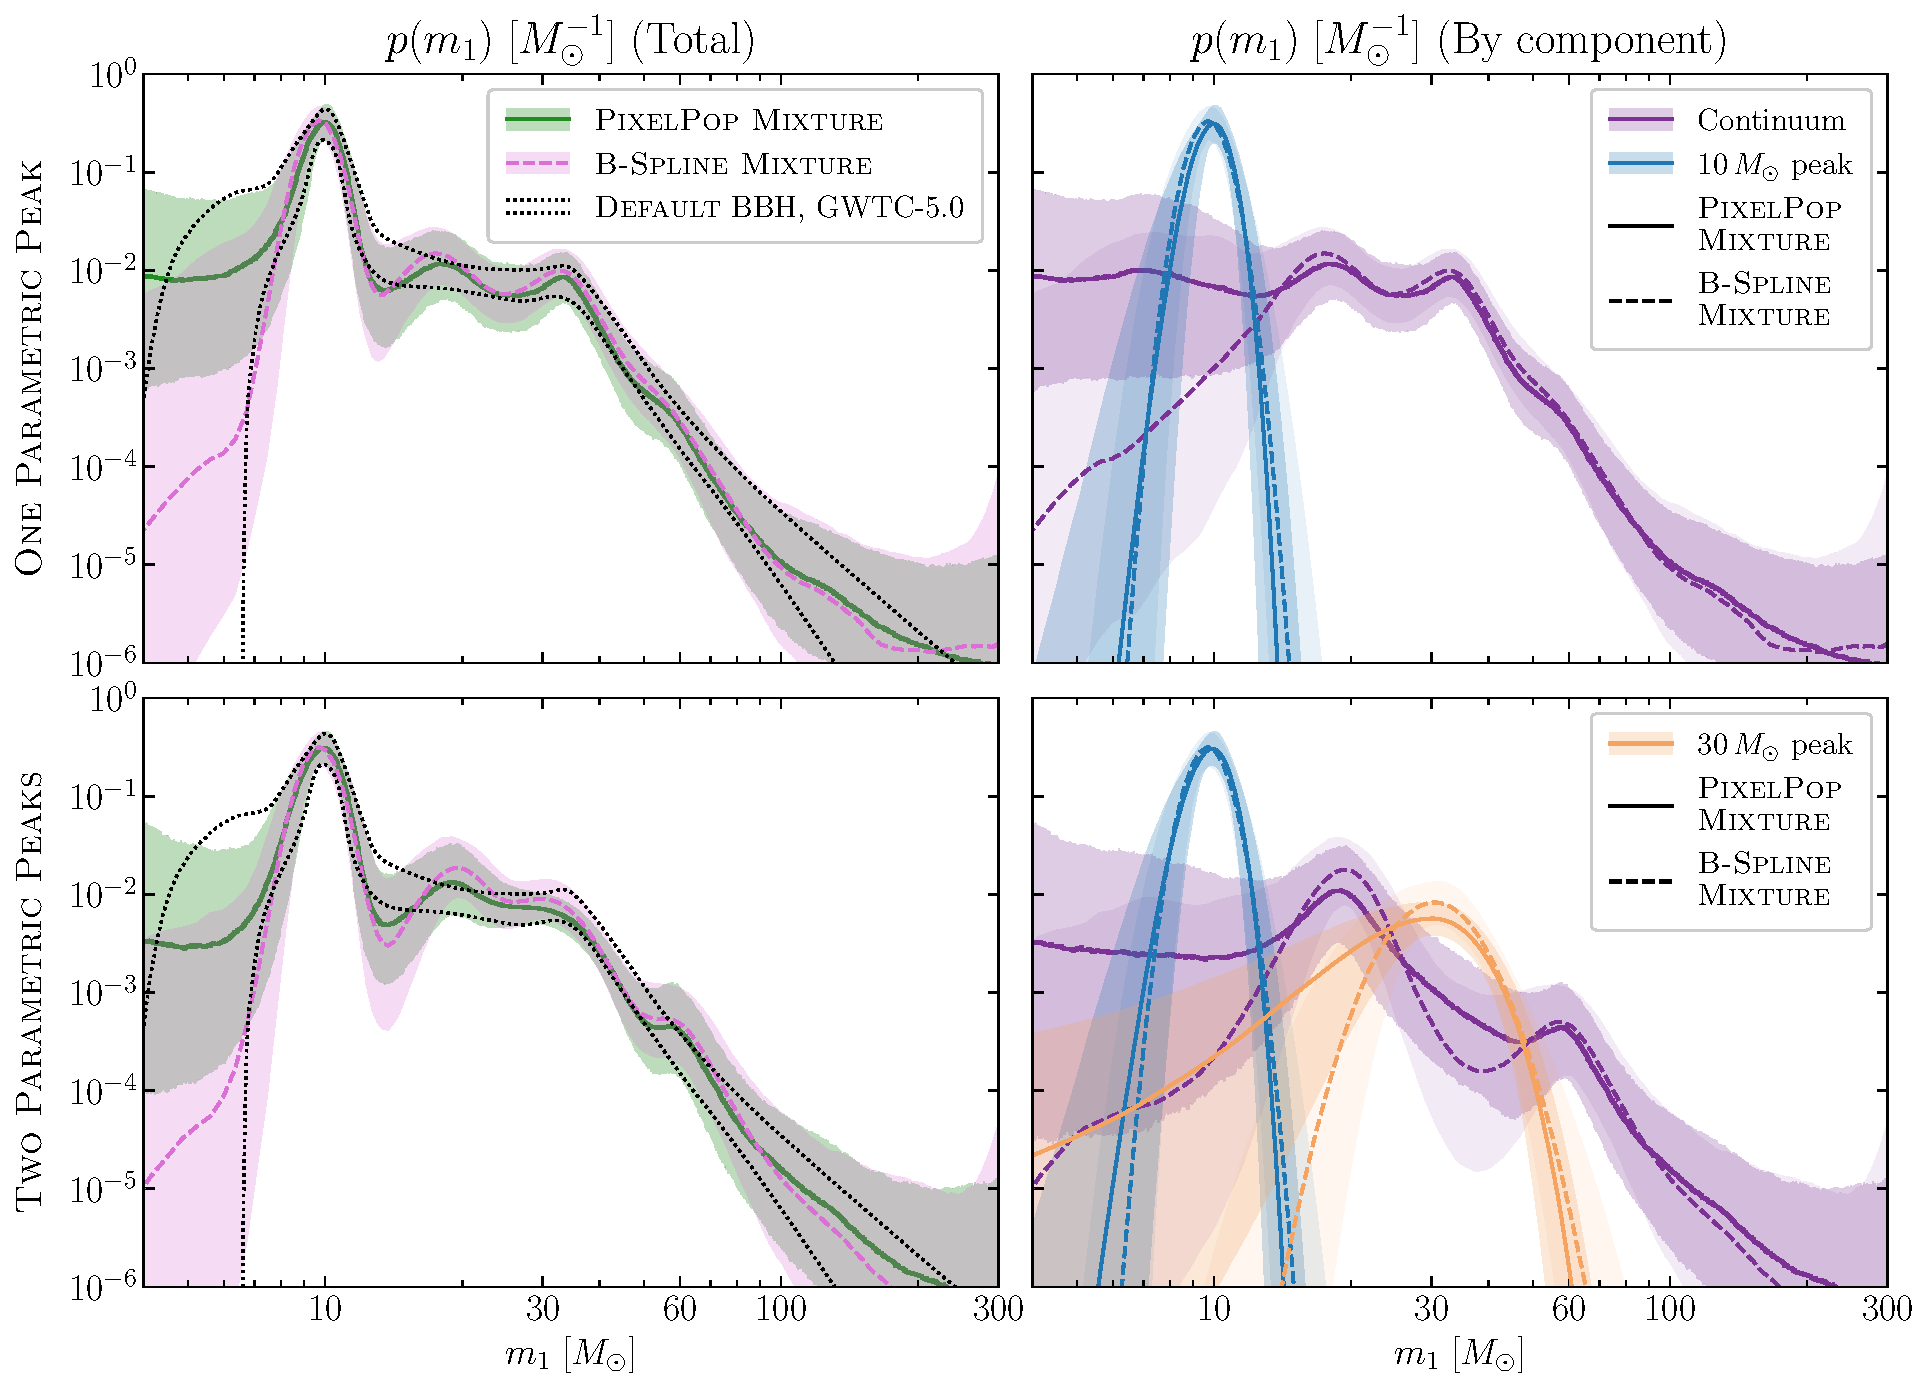
\includegraphics[width=\linewidth]{plots/m1-ppd.pdf}
\caption{The distribution of primary mass of the \ac{BBH} population inferred with \PPMixture (green) and \GwinfMixture (pink) for the \oneparpeak and \twoparpeaks variants.  \textcolor{red}{Add more details, let me know if you have any suggestions!}
}
\label{fig:m1-ppd}
\end{figure*}

\section{Results}\label{sec:results}

Figure~\ref{fig:m1-ppd} shows the primary-mass distribution inferred with the \oneparpeak (top) and \twoparpeaks (bottom) variants.
The left panels show the total distribution, $p(m_1)$, inferred with \PPMixture and \GwinfMixture, along with the distribution obtained with the \textsc{Default} BBH model from \ac{GWTC-5}~\citep{LIGOScientific:2026ctl}. The right panels show the individual components of both mixture models.

In both variants, we find striking agreement between \PPMixture and \GwinfMixture, despite the significantly different modeling assumptions adopted for each model.
Both methods recover the global peak near \textcolor{red}{$10\,\Msun$}, as well as features with similar locations and amplitudes near \textcolor{red}{$20\,\Msun$} and \textcolor{red}{$60\,\Msun$}.
While the inferred distributions are broadly consistent with the \ac{GWTC-5} \textsc{Default} \ac{BBH} model, additional structure is more clearly visible in our mixture models.

With \oneparpeak, the continuum recovers two excesses near $20\,\Msun$ and $30\,\Msun$, along with a less pronounced feature near $60\,\Msun$.
When we model the $30\,\Msun$ feature parametrically with \twoparpeaks, the structure near $60\,\Msun$ becomes more prominent in the continuum of both mixture models (bottom right panel).
To test whether this feature corresponds to a local maximum, in

\begin{figure*}
\centering
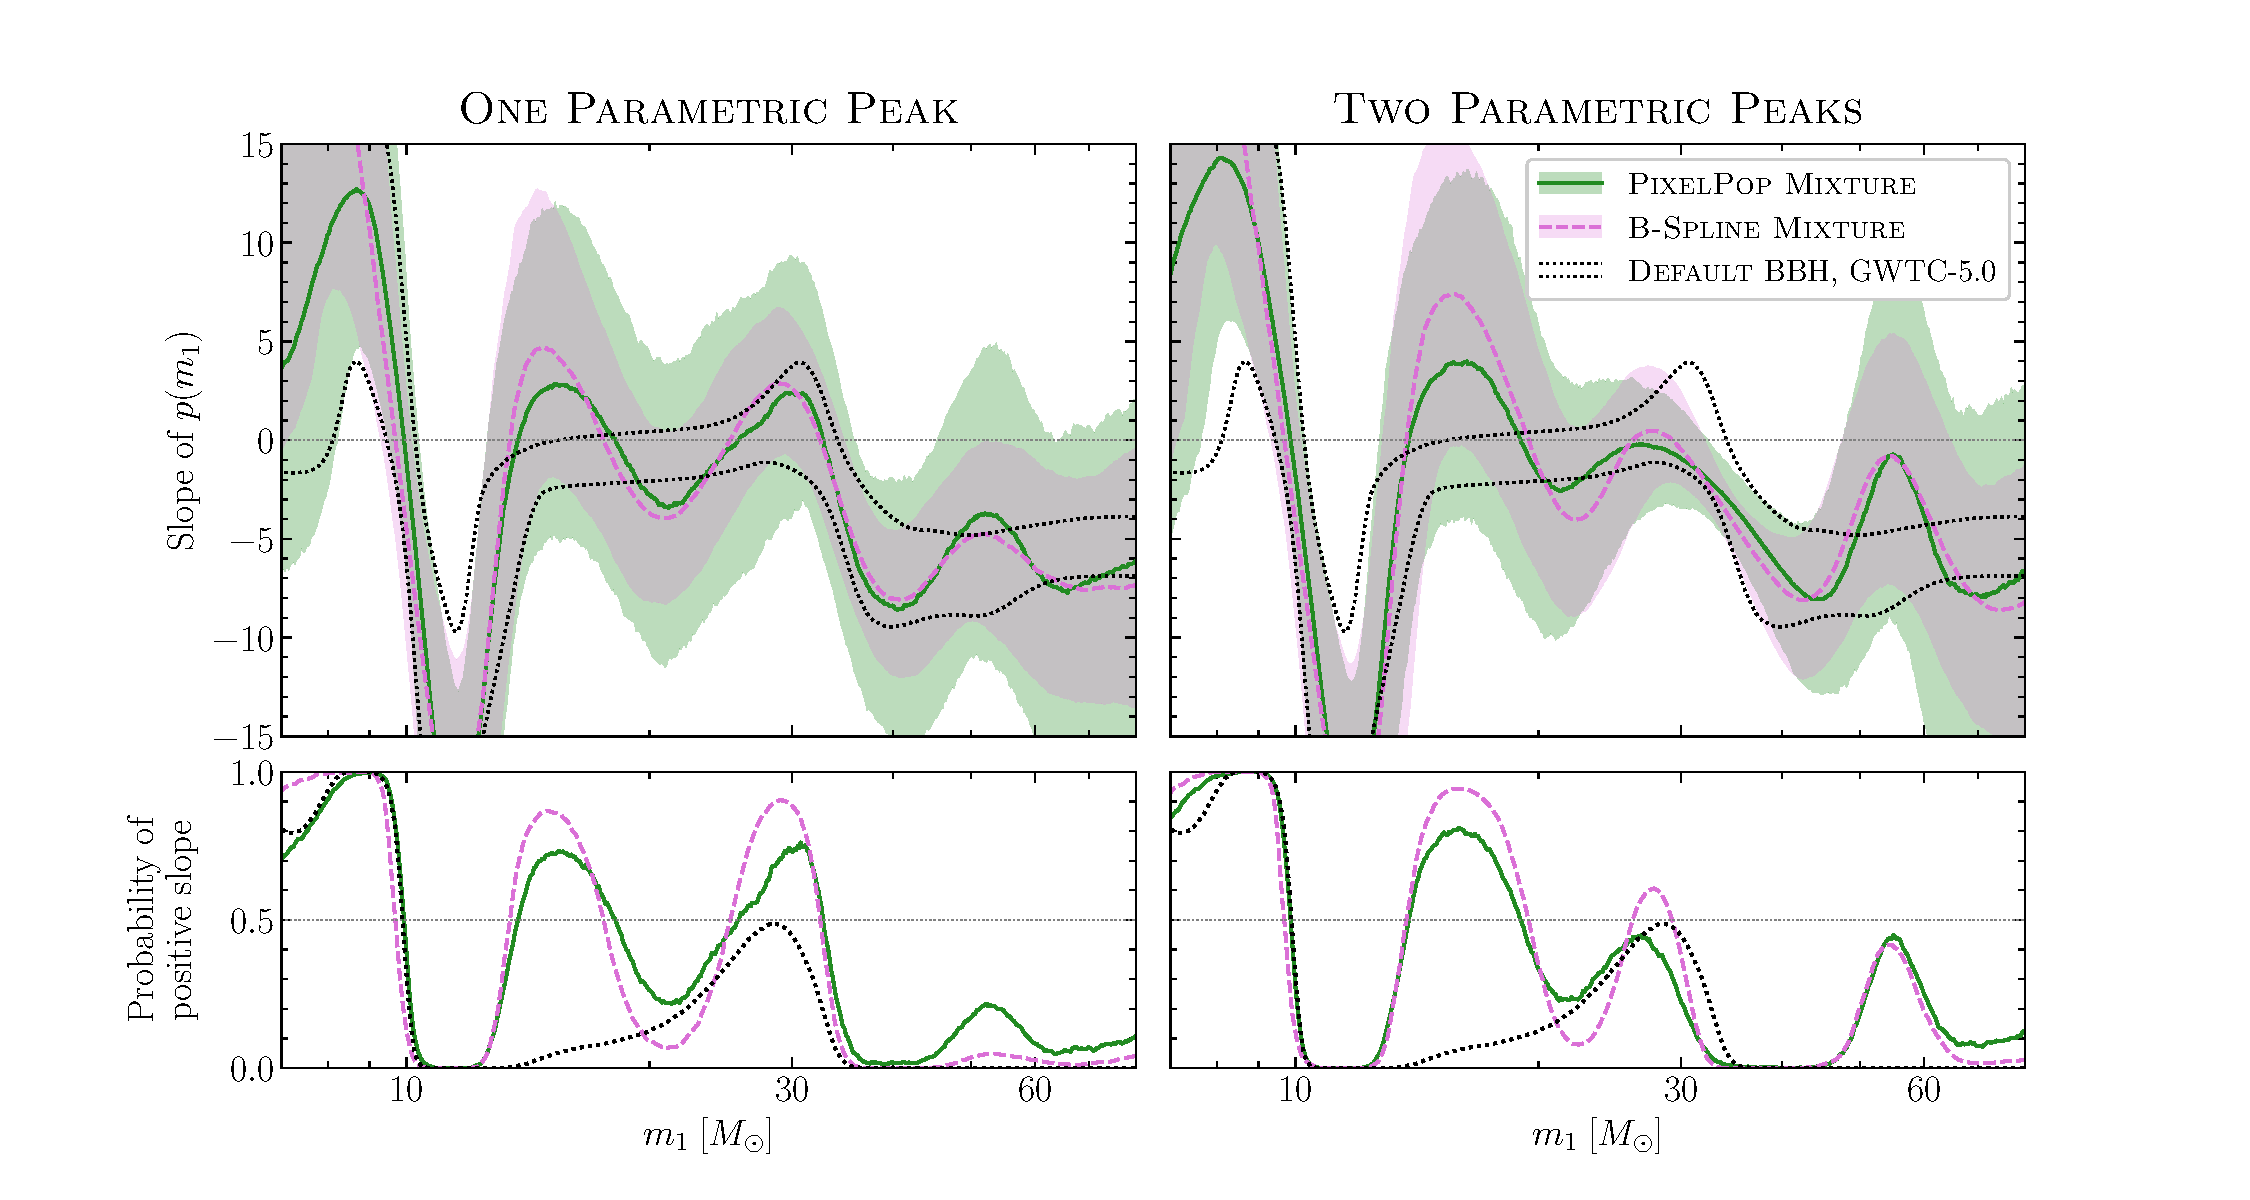
\includegraphics[width=\linewidth]{plots/m1-derivatives.pdf}
\caption{\textcolor{red}{This is the derivative $d \ln p(m_1)/d \ln m_1$ and the probability that it is larger than zero.}
}
\label{fig:m1-derivative}
\end{figure*}

We also find good agreement in the inferred mixing fractions.
With \oneparpeak, we infer a continuum mixing fraction of \textcolor{red}{$\xi_c=0.36^{+0.21}_{-0.12}$} (90\% symmetric credible interval) for \PPMixture and \textcolor{red}{$\xi_c=0.29^{+0.19}_{-0.13}$} for \GwinfMixture.
With \twoparpeaks, the continuum fractions decrease to \textcolor{red}{$\xi_c=0.19^{+0.17}_{-0.09}$} and \textcolor{red}{$\xi_c =0.17^{+0.16}_{-0.08}$}, respectively.
Both mixture models also recover consistent mixing fractions for the feature near $30\,\Msun$ in \twoparpeaks. We measure \textcolor{red}{$\xi_{30\,\Msun}=0.14^{+0.07}_{-0.05}$} (\PPMixture) and \textcolor{red}{$\xi_{30\,\Msun}=0.15^{+0.09}_{-0.06}$} (\GwinfMixture).

To characterize the nature of the features recovered by our two models in both \oneparpeak and \twoparpeaks, we examine the slope of the primary-mass distribution, $\mathrm{d}\ln p(m_1)/\mathrm{d}\ln m_1$, across posterior realizations.
We compute the derivative over an interval $\Delta \ln m_1 \approx 0.15\,\Msun$, and calculate the posterior probability that it is positive. Our result is robust to different choices of \textcolor{red}{$\Delta \ln m_1 \in [XX, YY]$}.

Figure~\ref{fig:m1-derivative} shows the inferred derivatives of $p(m_1)$ (top panels) and the corresponding probabilities of a positive slope (bottom panels), for \oneparpeak (left) and \twoparpeaks (right) as a function of mass. We also show the same quantities for the \ac{GWTC-5} \textsc{Default} \ac{BBH} model for comparison.

In both variants, the only clearly resolved transition from positive to negative slope occurs near $10\,\Msun$, corresponding to the global maximum of the primary-mass distribution. 
At $\sim20\,\Msun$, however, both mixture models show \emph{suggestive} evidence for an additional local maximum. 
With \oneparpeak, the posterior probability of a positive slope is approximately $\textcolor{red}{70\%}$ ($\textcolor{red}{85\%}$) near $\textcolor{red}{15\text{--}16\,\Msun}$, before decreasing to $\textcolor{red}{30\%}$ ($\textcolor{red}{10\%}$) by $\textcolor{red}{20\text{--}21\,\Msun}$, for \PPMixture (\GwinfMixture).
We find a similar trend with \twoparpeaks, where the probability decreases from approximately $\textcolor{red}{80\%}$ ($\textcolor{red}{90\%}$) near $\textcolor{red}{16\,\Msun}$ to $\textcolor{red}{30\%}$ ($\textcolor{red}{10\%}$) near $\textcolor{red}{21\text{--}22\,\Msun}$. 

%The evidence for a local maximum near $30\,\Msun$ is more sensitive to the modeling assumptions.
% With \oneparpeak, both \PPMixture and \GwinfMixture show suggestive evidence for a local maximum. The probability of a positive slope is approximately $\textcolor{red}{75\%}$ and $\textcolor{red}{90\%}$, respectively, near $\textcolor{red}{27\text{--}29\,\Msun}$, decreasing to nearly zero by $\textcolor{red}{35\text{--}40\,\Msun}$.
% This support is stronger than that found with the \ac{GWTC-5} \textsc{Default} \ac{BBH} model, for which the probability of a positive derivative is only $\textcolor{red}{50\%}$ near $\textcolor{red}{30\,\Msun}$ before decreasing to nearly zero.
% With \twoparpeaks, however, the support for a positive slope reduces: the maximum probabilities of a positive slope below $30\,\Msun$ decrease to approximately $\textcolor{red}{45\%}$ and $\textcolor{red}{60\%}$ for \PPMixture and \GwinfMixture, respectively.

The evidence for a local maximum near $30\,\Msun$ is more sensitive to the modeling assumptions. With \oneparpeak, both \PPMixture and \GwinfMixture show suggestive evidence for a local maximum, with probabilities of a positive slope of approximately $75\%$ and $90\%$, respectively, just below the feature, decreasing to nearly zero around $\textcolor{red}{35\text{--}40\,\Msun}$. This support is stronger than that found with the \ac{GWTC-5} \textsc{Default} \ac{BBH} model, for which the probability of a positive slope is $\sim50\%$ at best. With \twoparpeaks, however, these probabilities decrease to approximately $45\%$ and $60\%$, respectively.

The weaker evidence for a local maximum with \twoparpeaks does not necessarily imply the absence of such a feature in the underlying astrophysical population.
Instead, it may be a consequence of how the feature is modeled parametrically.
In \PPMixture, the Gaussian component may broaden to accommodate additional structure rather than requiring more complex features in the \PixelPop continuum, consistent with an Occam's razor preference for a simpler description of the data~\citep{Alvarez-Lopez:inprep}.
In \GwinfMixture, a peak-like feature near \(30\,\Msun\) is captured by the continuum component in \oneparpeak.
By introducing a second peak component as in \twoparpeaks, we also introduce degeneracies in the regime where the continuum and \(30\,\Msun\) overlap, as shown in the bottom right panel of Fig. \ref{fig:m1-ppd}.
% In B-splines, we also introduce more dimensions (since we have an additional component in 2 peaks with more ratio and spin PPDs. We are reaching the limit of variance cuts, so this broadening feature could be a result of a reduced maxL because of an increase in hyperparameters being sampled.
% consequence on the limit of the likelihood uncertainty. 

\begin{figure*}
\centering
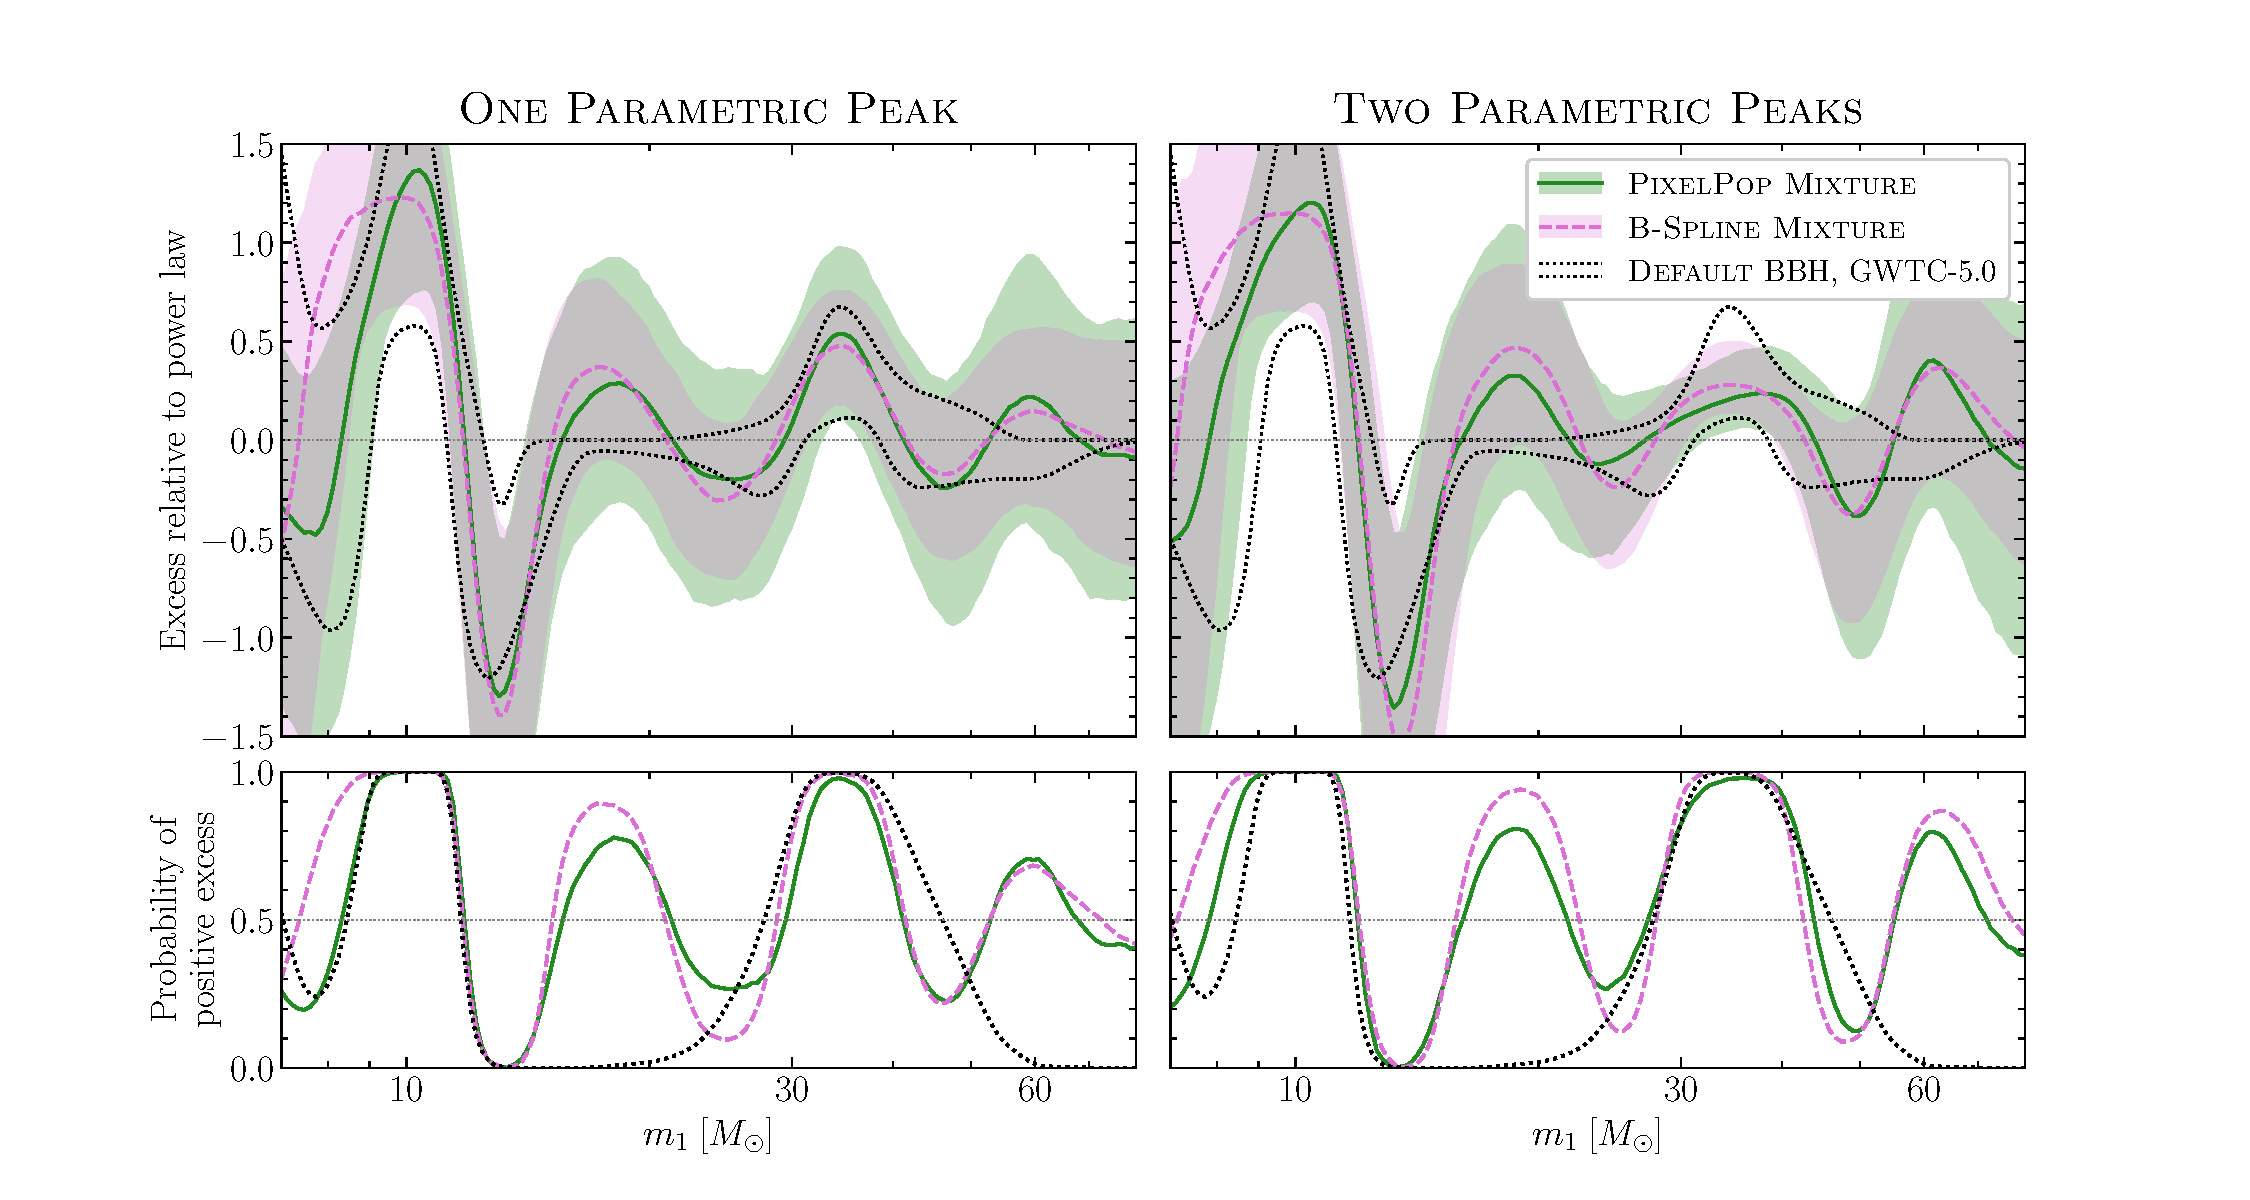
\includegraphics[width=\linewidth]{plots/m1-excess.pdf}
\caption{\textcolor{red}{This shows the excess relative to a power law for each hyperposterior draw. For each mass, I define three windows: one on the left \(L\), one on the right \(R\), and a central window \(C\). I then use \(L\) and \(R\) to calculate what a power law passing through \(C\) would look like and how much excess there is in each hyperposterior draw. The top row shows the posterior on the excess, while the bottom row shows the probability of a positive excess as a function of mass.}
}
\label{fig:m1-excess}
\end{figure*}

At higher masses, modeling the feature near $30\,\Msun$ parametrically allows the continuum to describe additional structure, resulting in an increased probability of a positive derivative near $60\,\Msun$. In both \PPMixture and \GwinfMixture, the probability of a positive slope increases from nearly zero at $\textcolor{red}{40\text{--}45\,\Msun}$ to approximately $\textcolor{red}{40\%}$ at $\textcolor{red}{55\text{--}60\,\Msun}$, before decreasing to $\textcolor{red}{5\text{--}10\%}$ above $\textcolor{red}{65\,\Msun}$. This is substantially higher than with \oneparpeak, where the maximum probabilities of a positive slope are $\textcolor{red}{20\%}$ and $\textcolor{red}{5\%}$ for \PPMixture and \GwinfMixture, respectively. While we do not find strong evidence for a local maximum near $60\,\Msun$, the inferred slopes suggest additional structure in this region.

The derivative analysis provides suggestive evidence for local maxima, but not all the features we recover necessarily correspond to distinct peaks.
We therefore investigate these features further by testing for excesses relative to a power law in the primary-mass distribution.

For each hyperposterior draw, we consider three neighboring mass intervals of equal width in $\ln m_1$ across the entire mass range. We compare the average density in the central interval with the mean of the densities in the two surrounding windows, which provides the expected probability density for a power law between those two points. We then calculate the probability of an excess relative to this power law as a function of mass. Our results are robust to the choice of interval width. 

Figure~\ref{fig:m1-excess} shows the inferred excesses relative to a power law (top panels) and the corresponding probabilities of a positive excess (bottom panels), for \oneparpeak (left) and \twoparpeaks (right). We also show the same quantities for the \ac{GWTC-5} \textsc{Default} \ac{BBH} model for comparison.

Near $20\,\Msun$ and $60\,\Msun$, both \PPMixture and \GwinfMixture find suggestive evidence for an excess, with higher probabilities in \twoparpeaks than in \oneparpeak. Near $20\,\Msun$, the probabilities increase from approximately $\textcolor{red}{70\text{--}90\%}$ with \oneparpeak to $\textcolor{red}{80\text{--}95\%}$ with \twoparpeaks. Similarly, near $60\,\Msun$, they increase from approximately $\textcolor{red}{75\%}$ ($\textcolor{red}{70\%}$) to $\textcolor{red}{80\%}$ ($\textcolor{red}{90\%}$) for \PPMixture (\GwinfMixture). In contrast, the \ac{GWTC-5} \textsc{Default} \ac{BBH} model shows no support for an excess in either region. The higher probabilities for an excess with \twoparpeaks may reflect the additional freedom of the continuum to describe these features when the structure near $35\,\Msun$ is modeled parametrically. 

Near $30$--$35\,\Msun$, both mixture models find probabilities of a positive excess close to $\textcolor{red}{100\%}$ in both variants, including \twoparpeaks, where the evidence for a local maximum in Fig.~\ref{fig:m1-derivative} is weaker. The \ac{GWTC-5} \textsc{Default} \ac{BBH} model confidently recovers an excess in this region. Although the nature of this feature remains uncertain, our results confirm the presence of additional structure at this mass scale, in agreement with previous studies~\citep[e.g.,][]{Talbot:2018cva, LIGOScientific:2018jsj, LIGOScientific:2020kqk, KAGRA:2021duu, Farah:2023vsc,Roy:2025ktr, Sridhar:2025kvi,LIGOScientific:2026ctl}.

%We also calculate the joint probability of finding excesses near both $20$ and $30$--$35\,\Msun$ within the same hyperposterior realization. We find probabilities of $89\%$ ($95\%$) with \oneparpeak and $92\%$ ($97\%$) with \twoparpeaks, for \PPMixture (\GwinfMixture). In contrast, the \ac{GWTC-5} \textsc{Default} \ac{BBH} model gives a probability of only $6\%$. These results suggest that the primary-mass distribution likely contains two separate features near $20$ and $30$--$35\,\Msun$, rather than a single broad excess.

\section{Discussion}

\begin{itemize}
    \item Our results still allow for a powerlaw (And even a dip!) at 20 and 60 Msun. This is most likely not the case because we still find suggestive evidence for peaks, but it's important to emphasize that we'll need more observations to determine the significance of these features and better characterize their shapes.
    \item Potential origin of these features?
\end{itemize}

Figure~\ref{fig:q-chieff-ppd} shows the mass ratio and effective spin distributions inferred with the \oneparpeak (top) and \twoparpeaks (bottom) variants.
The \(10\,\Msun\) component is consistent with isolated binary formation, where mass ratios are expected to be consistent with \(q\sim1\) and spins are preferentially aligned with the orbital angular momentum.
 
\cite{Legred:2026oiz} argues that the \(10\,\Msun\) peak comes from a subpopulation of failed supernovae~\citep{Disberg:2023gel}; they explicitly model a gap in the primary mass distribution.
A pileup of \red{merger rates} near the \(10\,\Msun\) peak \red{may lead to} a dearth in BBHs up until the \(\sim20\,\Msun\) feature.
Mergers that populate past this gap could originate from hierarchical mergers, as suggested by \cite{Tong:2025xir} and \cite{Plunkett:2026pxt}.
Fig.~\ref{fig:m1-excess} hints at this feature, as the excess dips below the \ac{GWTC-5} \textsc{Default} \ac{BBH} model.

Hierarchical mergers past \(m_1\sim45\,\Msun\) could populate the forbidden region predicted by pair instability supernovae~\citep{Tong:2025wpz, Antonini:2025ilj}.
Plateau feature in \twoparpeaks around \(60\,\Msun\), suggestive of \cite{Antonini:2024het} and \cite{Antonini:2022vib}, and the CIs in the derivative analysis at this mass do not rule out a plateau-like feature that would indicate the \red{beginning of the contribution of} hierarchical mergers to the primary mass distribution.

\section*{Acknowledgements}
\begin{acknowledgments}
\textcolor{red}{We thank friends for discussions.}
%
S.A.-L. is supported by the Andrei Sakharov Physics Fellowship Fund at MIT and NSF grant No. PHY-2045740. 
%
B.F. and I.J.R. acknowledge support from the National Science Foundation under grant PHY-2146528.
\textcolor{red}{Please add your funding!}
%
The authors are grateful for computational resources provided by the LIGO Laboratory and supported by National Science Foundation Grants PHY-0757058 and PHY-0823459.
%
This research has made use of data or software obtained from the Gravitational Wave Open Science Center (gwosc.org), a service of the LIGO Scientific Collaboration, the Virgo Collaboration, and KAGRA,
%
and is based upon work supported by NSF's LIGO Laboratory, which is a major facility fully funded by the National Science Foundation.
\end{acknowledgments}

\appendix 


\section{Model details}\label{app:model-details}

For events in \acs{GWTC-3} and earlier catalogs, we use posterior samples generated with the \textsc{IMRPhenomXPHM} waveform model~\citep{Pratten:2020ceb}.
For events in \acs{GWTC-4} and \acs{GWTC-5}, we use \textsc{NRSur7dq4} samples when available and \textsc{IMRPhenomXPHM-SpinTaylor} samples otherwise.
Although our waveform choices differ slightly from those of~\citet{LIGOScientific:2026wfs}, they increase the number of posterior samples per event from \textcolor{red}{1993} to 6913, reducing the parameter-estimation contribution to the log-likelihood variance.

We account for selection effects by computing sensitivity estimates for \acs{BBH} systems over O1--O4b via a simulation campaign~\citep{Essick:2025zed,ligo_scientific_collaboration_2026_19500052}.
We evaluate the population likelihood using Monte Carlo integration and limit the variance of the log-likelihood estimate to be less than one during inference~\citep{Tiwari:2017ndi,Essick:2022ojx,Talbot:2023pex,Heinzel:2025ogf}.

\begin{itemize}
    \item Describe \PixelPop: normalized version, ICAR prior, uniform mixing fraction, marginalized over sigma, etc.
    \item Describe parametric models and priors, etc. Particularly for \gtwou, it's flexible enough.
\end{itemize}

For \PPMixture, we model the $m_1$ continuum with \PixelPop and its mass ratio ($q$) and effective spin (\chieff) distributions parametrically.
The full \PPMixture model is given by

\begin{widetext}
\begin{equation}\label{eq:pp-mixture}
  p_{\rm mix}^{\rm PP}(m_1,q,\chieff) =
  \xi_c\,p_{\rm PP}(m_1)\,
  p_{\rm c}(q\,|\,m_1)\,p_{\rm c}(\chieff) +
  (1-\xi_c)\sum_{i=1}^{N_{\rm p}}
  \lambda_i\,p_{{\rm peak},i}(m_1)\,p_{i}(q\,|\,m_1)\,p_{i}(\chieff),
\end{equation}
\end{widetext}

where $\xi_c$ is the fraction of binaries in the \PixelPop component and $\lambda_i$ are the relative weights of the $N_{\rm p}$ parametric peaks, with $\sum_i \lambda_i = 1$.
For \oneparpeak, $N_{\rm p}=1$ and $\lambda_1=1$; for \twoparpeaks, $N_{\rm p}=2$.

To model each peak, we use a Gaussian in $m_1$.
We restrict the means of the $10\,\Msun$ and $30\,\Msun$ peaks to $[8, 12]\,\Msun$ and $[25, 40]\,\Msun$, respectively, to avoid degeneracies between the peaks.
The effective spin and mass ratio distribution of each peak are also Gaussian, with $q$ truncated to $m_2 \geq 3\,\Msun$.

To model the continuum, we use a one-dimensional \PixelPop field with 1000 bins uniform in $\ln m_1$ over $[3,300]\,\Msun$.
We use a mass-independent \gtwou model for the effective spin (see~\cite{Alvarez-Lopez:2026ymo}), which consists of a mixture of a Gaussian bulk and two half-uniform components on either side of $\chieff = 0$.
This model allows for structure beyond a single Gaussian, providing flexibility to describe the combined spin distribution of the $30\,\Msun$ feature alone (in \twoparpeaks) and when modeled with the rest of the continuum (in \oneparpeak).
In \twoparpeaks, we use a Gaussian for the mass ratio distribution.
In \oneparpeak, we use a mixture of two Gaussians, since the continuum also includes the $30\,\Msun$ feature, whose mass ratios may differ from those of the rest of the continuum.
In both cases, we apply the same $m_2$ truncation as for the $q$ distributions of the peaks.

We infer the \ac{BBH} merger rate $\mathcal{R}(m_1,q,\chieff;z)
= R_0\,(1+z)^\kappa\, p_{\rm mix}^{\rm PP}(m_1,q,\chieff)$, where the redshift distribution evolves as a powerlaw with index $\kappa$~\citep{Fishbach:2018edt} and $R_0$ is the overall merger-rate scale.

The full \GwinfMixture model is given by
\begin{widetext}
\begin{equation}\label{eq:bspline-mixture}
\begin{aligned}
    p_\mathrm{mix}^\mathrm{BS}(z,m_1,q,a_1,a_2,\cos\theta_1,\cos\theta_2)&=p(z)\left[\xi_cp_c(m_1)p_c(q|m_1)p_c(a_1)p_c(a_2)p_c(\cos\theta_1)p_c(\cos\theta_2)\vphantom{\sum_{i=1}^{N_p}}\right. \\
    &\left.+\sum_{i=1}^{N_p}\xi_ip_{\mathrm{peak},i}(m_1)p_i(q|m_1)p_i(a_1)p_i(a_2)p_i(\cos\theta_1)p_i(\cos\theta_2)\right],
\end{aligned}
\end{equation}
\end{widetext}
where \(\xi_c,\,\xi_i\) are the fractions of binaries in the continuum and peaks of the \GwinfMixture, respectively.
With the exception of the shared redshift distribution and the peaks in the primary mass distribution, every distribution is modeled \ij{by/with/using} cubic B-splines.
The \GwinfMixture models the component spins of the binary as independent and identically distributed (IID).
\ij{Again}, for \oneparpeak, \(N_\mathrm{p}=1\); for \twoparpeaks, \(N_\mathrm{p}=2\).

Each peak is modeled with a log-Gaussian in \(m_1\), where the log-means \(\ln(M/M_\odot)\) of the \(10\,M_\odot\) and \(30\,M_\odot\) peaks are constrained to \([\ln7,\ln15]\) and \([\ln28,\ln40]\) respectively.

The shared redshift distribution follows a modulated power-law distribution (in linear \(z\)) as in \cite{Edelman:2022ydv}:
\[
p(z)=\frac{dV_c}{dz}(1+z)^{\kappa-1}\exp\mathcal{B}(z),
\]
where \(dV_c\) denotes the differential co-moving volume and \(\mathcal{B}(z)\) denotes a B-spline.

\sa{@Ivan, can you please fill the rest of this section with the implementation details of the B-splines? Also make explicit the (many) differences with \PPMixture since it's really cool that despite the differences we get similar results.} 
\ij{Some differences can be pointed to in a table containing priors on the peaks?}

\begin{deluxetable*}{cccc}
\tablecaption{Summary of \PPMixture and \GwinfMixture model parameters and priors. \PPMixture models the peaks as linear-Gaussians, whereas \GwinfMixture models the peaks as log-Gaussians.}
\tablehead{
\colhead{Parameter} & \colhead{Description} & \colhead{\PPMixture} & \colhead{\GwinfMixture}
}
\label{tab:peak-parameters}
\startdata
$\mu_1$ & Location of the first peak & prior & $\mathcal{N}_{[\ln7, \ln15]}(\ln10, \ln5)$ \\
$\sigma_1$ & Width of the first peak & prior & $\mathcal{N}_{[0.04, 0.2]}(0, 0.2)$ \\
$\mu_2$ & Location of the second peak & prior & $\mathcal{N}_{[\ln28, \ln40]}(\ln35, \ln5)$ \\
$\sigma_2$ & Width of the second peak & prior & $\mathcal{N}_{[0.04, 0.3]}(0, 0.2)$ \\
$\xi_c, \lambda_i$ & \PPMixture mixing fractions & prior & - \\
$\xi_c, \xi_i$ & \GwinfMixture mixing fractions & - & ${\rm Dir}(\mathbf{\alpha}=(1,1,1))$ \\
\enddata
\end{deluxetable*}
The priors on the parametric peaks are given in Table~\ref{tab:peak-parameters}.

\section{Other plots and corner plots}

Including mass ratio.

\sa{Maybe show the mixing fraction plot? Probably not necessary}

\section{Rates comparison}\label{app:rates}

\section{Two-dimensional \PPMixture models}\label{app:2d-pp-mixture}

Only in primary mass and mass ratio space. Spin analyses we leave for future work. 

\sa{Potentially other model variations? Like maybe show that the same things hold (approximately) even when q and spin are shared in PP? }

\sa{Also maybe using less bins in 1D? Like 100 bins, to show that it's not a resolution effect from 2D PixelPop?}

\bibliography{draft}
\bibliographystyle{aasjournal}


\end{document}
